\documentclass[a4paper,10pt]{article}
\usepackage[utf8]{inputenc}

% increase margins
\usepackage{fullpage}
\usepackage[left=1in,top=1in,right=1in,bottom=1in,headheight=3ex,headsep=3ex]{geometry}

% this puts two lines between paragraphs and no indent
\usepackage[parfill]{parskip}

% set up colors
\usepackage{array, xcolor}
\usepackage{color,hyperref}
\usepackage{graphicx}

\definecolor{torontoblue}{HTML}{00204E}
\definecolor{linkblue}{HTML}{0000FF}

% define hyperlink style
\hypersetup{colorlinks,breaklinks,
            linkcolor=linkblue,urlcolor=linkblue,
            anchorcolor=linkblue,citecolor=linkblue}


%opening
\title{Weekly Journal}
\author{Leila Uy}



\begin{document}

\maketitle

\section{Work Update}
I will be writing this journal afternoon of Monday, so it might be bit oudated depending on what I accomplish Monday night.

\subsection{Parallel R}
So as we know, the previous code I thought accomplished parallel kmeans is flawed. Therefore, we have to find a different way for the kmeans function. For mask, we have a code that I pushed to the repo on my working branch that has a parallelization of mask using snow. Looking at the CPU utilization, we can see it is running on all CPUs.
\begin{figure}[h!]
    \caption{A sudden jump in all CPUs while testing the parallel mask}
    \centering
    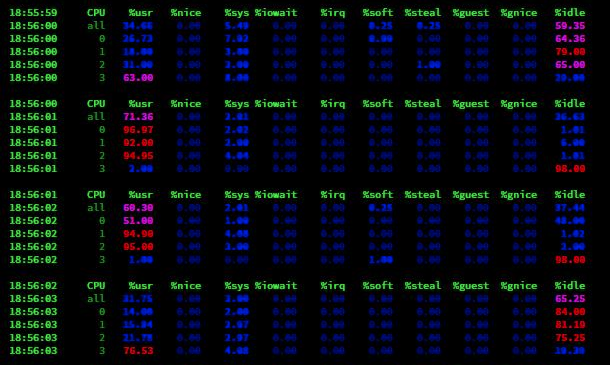
\includegraphics[scale=0.5]{mask-CPU-util.png}
\end{figure}

I need to test the speed for the process with large data sets, so I will do that tonight.

\subsection{Data Upload - possible BASH script}
Diljot and Valerie are currently struggling with the upload speeds into S3 buckets, and they expressed their interest in using the instances for this task. Therefore, I will try working on a base script for the two to use in an EC2 instance to directly upload to S3 bucket. I will try to update during the meeting.

\subsection{Parallel GRASS}
I'm currently learning GRASS scripting in my free-time because I need to dust off my BASH skills. I don't know if I will get to learn everything I need to accomplish parallelization in GRASS before next week, but I might use this as a contingency for next semester. You can see me struggle through \hyperlink{https://github.com/Leila-U/GRASS-bash}{my personal repo.}

\section{Literature Review}
I have changed my literature focus on Ontario agriculture and I found the topic that you brough up last week about farmers moving Northern due to climate change interesting. Research by Chapagain \cite{chapagain2017farming} seems to suggest that there is untapped potential in Northern Ontario farming and although there are several barriers like extreme climate conditions, labor shortages, and insufficient infrastructure, the change of cliamte could actually open opportunities. For example, increased annual precipitation and rising temperatures. The northern latitude also provides extensive summer sunshine by those in the west and creates favourable conditions for fruit crops, bioenergy crops and oilseed crops. Finally, it promotes new practices that are only used in Northeastern Ontario sometimes.

So, what happens to the conditions of current Canadian agriculture areas? While there is little consensus about the possibilities, it is expected that most regions in Canada will have longer frost-free seasons and increased evapo-transpiration rates and moisture deficits. This might be favorable for some agriculture like apply and grape producers in the British Columbia interior. Of course, these benefits could be offset by extreme heat events, increased persistance of crop pests through milder witners, and anticipated ater supply challenges. \cite{reid2007vulnerability}

% this info creates the bibliography
% YOU WILL NEED TO CHANGE THIS PATH TO THE LOCATION OF THE BIB file
\bibliography{./agclimate.bib}
\bibliographystyle{plain}


\end{document}
